\documentclass{article}

\usepackage{amsmath}
\usepackage{amssymb}
\usepackage{graphicx}
\usepackage{epigraph}

\title{Phylourny: a new way of looking at tournament predictions}
\author{Ben Bettisworth}
\begin{document}

\newcommand{\beats}[2]{P_{#1 \vdash #2}}

\maketitle
\epigraph{Amongst all unimportant subjects, football is by far the most important.}{Pope John Paul II}
\section{Introduction}

Prediction of bracket based tournaments can be computationally expensive if a high degree of accuracy is desired. To
fully (and naively) evaluate the probability of the any particular tournament competitor placing, a high degree
polynomial must be evaluated. For a tournament with $n$ teams, a polynomial of degree up to $n$ must be evaluated. If
one wants to do this for every competitor in the tournament, then $n$ of these polynomials must be evaluated.
Alternatively, simulations used to estimate the distribution of winners for a tournament, which can be more efficient
computationally. However, such efficiency comes at a cost to the fidelity of the results.

However there is a similar problem in the field of computational phylogenetics which bears many similarities to the
problem of computing winning probabilities for a tournament. Some of the similarities are plain, such as both are often 
represented by a directed acyclic graph (DAG). But there are even deeper similarities, for example both use DAGs which
are limited to nodes with either in-degree 2 or 0.

Furthermore, both are based on statistical principles. Computational phylogenetics seeks to compute a likelihood, which
is the probability of a model, given some data. So, while this is in principle different than just computing a
probability, the actual computation is very similar. More importantly, the computation of the likelihood can be
expressed via polynomials, in almost the same fashion that computing the probability of a particular competitor winning a
tournament can be expressed. This common framework allows us to adapt techniques which have been developed to compute
phylogenetic likelihoods to instead compute the winner probabilities given a tournament.

Here we propose a novel method of computing win probabilities for a multi-elimination tournament, which combines the
fidelity of exact calculations with the speed of simulations. This new method, which we call Phylourny, is based on an
observation in Yang \textbf{CITE YANG} about the Felsenstien algorithm. Yang points out that Felsenstien's algorithm can
be thought of as an efficient way of computing polynomials of a high degree. 

\section{Background}

\begin{figure}
  \centering
  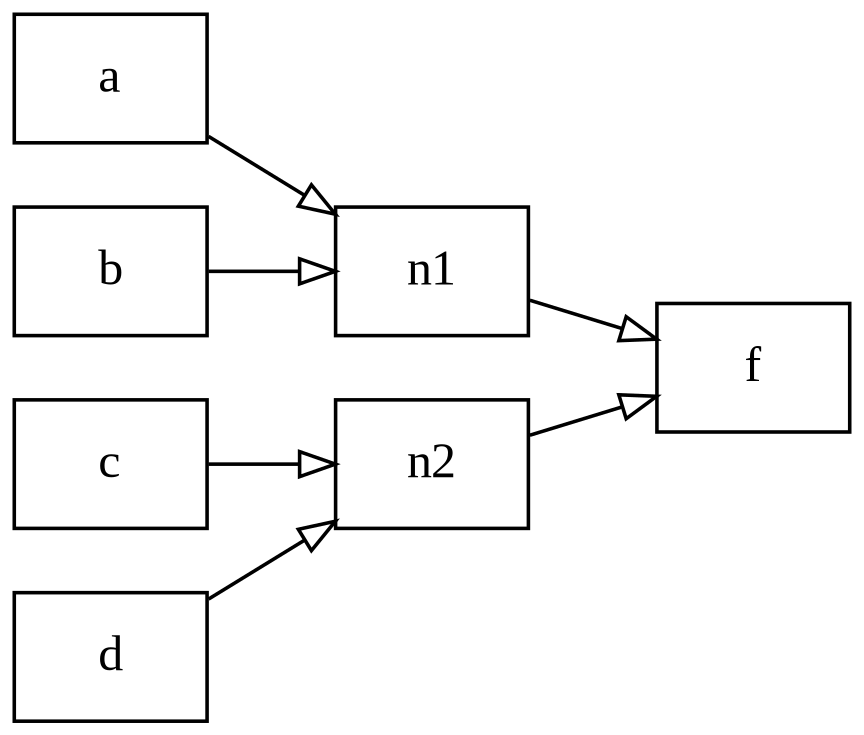
\includegraphics[width=\textwidth]{single-elim.png}
  \caption{A simple example tournament}
  \label{fig:single-elim}
\end{figure}

\begin{figure}
  \centering
  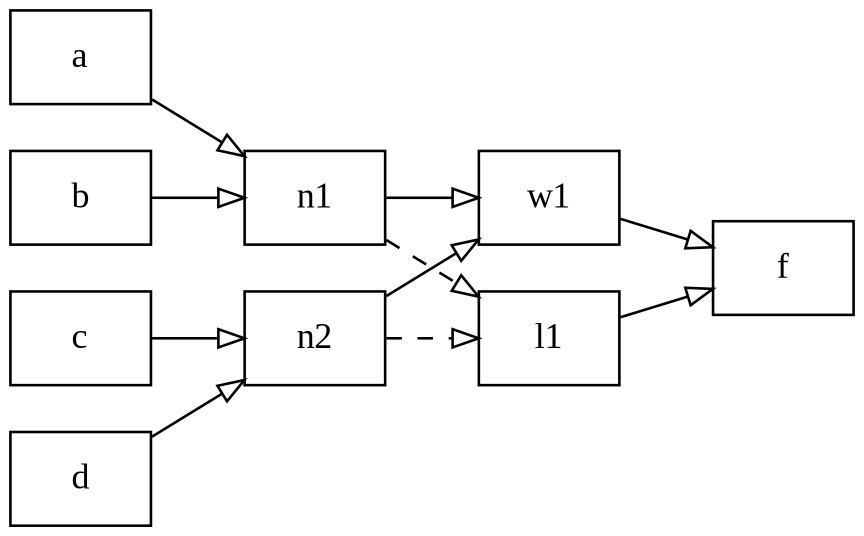
\includegraphics[width=\textwidth]{double-elim.png}
  \caption{A simple double elimination tournament}
  \label{fig:double-elim}
\end{figure}

\section{Method}

First, we will discuss the theory behind the computation of the single match's distribution of winners in the theory
section. Then, we will discuss how we use this theory to efficiently compute the distribution of winners for a general
tournament.

\subsection{Theory}

Some preliminary definitions. The win probability vector (WPV) for a given node is a vector containing the
probabilities of observing a competitor at that node. We denote the probability of team $a$ winning over team $b$ in a
single match as 

\begin{equation*}
\beats{a}{b}
\end{equation*}

which should be read as "the probability that team $a$ beats team $b$".

Suppose that we have a simple tournament, which is just two teams, $a$ and $b$. Then, the WPV which summarizes this
tournament is described by 

\begin{equation}
R_a = \beats{a}{b}, R_b = \beats{b}{a}
\label{eq:base}
\end{equation}

Because this is a trivial case, it is clear that the calculation is easy. For the interest of future examples though,
let us embellish this expression a little bit. First, lets introduce the WPVs for $a$ and $b$ as $w$ and $y$. Since $a$
and $b$ are "tips", we just set the probabilty of observing the team at that node to 1 for the team, and 0 everywhere
else. Then, we get the expression

\begin{equation}
R_a = (\beats{a}{b} \times y_a + \beats{a}{b} \times y_b) \times w_a.
\label{eq:embelished}
\end{equation}

We define $\beats{t}{t} = 0$ for any team $t$. So, because $\beats{a}{a} = 0$ and $y_b = 1$, we can reduce
Equation~\ref{eq:embelished} to Equation~\ref{eq:base}. Using this insight, we can build a general expression for the
WPV on a single elimination tournament as

\begin{equation}
  R_i = w_i \times \sum_{c\in C} \beats{i}{c} \times y_c.
\end{equation}

For multi-elimination tournaments, we need to account the fact that a competator can come from both sides of the
tournament. Therefore, we need to add a second term to the expression for the other side:

\begin{equation}
  R_i = \left(w_i \times \sum_{c\in C} \beats{i}{c} \times y_{c|i} \right) +
        \left(y_i \times \sum_{c\in C} \beats{i}{c} \times w_{c|i} \right).
        \label{eq:final}
\end{equation}

We calculate $w_{c|i} = w_{c}/(1 - w_i)$, and it should be thought of as the probability of observing competator $c$ at
$w$ given that competator $i$ is the other member of the match. So, Equation~\ref{eq:final} is the full general
expression for the WPV of a multi-elimination tournament. The final complication is that $\beats{a}{b}$ might be a "best
of $n$" series of matches, which will vary over the tournament (early matches are often only a "best of one", whereas
later matches might be a "best of 5"). This can be dealth with by computing a new $P'$ which is the pairwise probability
of winning the "best of $n$".

\subsection{Software}

To actually compute the WPV, we need to apply the expression in Equation~\ref{eq:final} to every node in the tournament. 
To do this, we can apply a version of Felsenstien's algorithm. Specifically, by computing the WPV for each node, we can
avoid recomputatation of any intermediate results, as the any given node's WPV only depends on its two children.

Felsenstien's algorithm is a method of computing statistical likelihoods of phylogenetic trees. Initially, it might not
seem like tournament probabilities and phylogenetic likelihoods are related, but some initial similarities are obvious.
First, both problems are based on structures called directed acyclic graphs or DAGs. Here, directed indicates that every
edge in the graph has a direction, and acyclic indicates that no cycles are present in the graph. 

\section{Results}

\section{Conclusion}

\end{document}
